%&template
\documentclass{article}
\usepackage{src/template}

\endofdump
\usepackage{minted}

\date{2026 -- 01 -- 04}
\useTemplate[NPA, Exercise=9]
\title{NPA -- Exercise 9}


\begin{document}
\maketitle
    
    \section{}
    \subsection{}

        Head-of-line blocking refers to the problem whereby a lost or delayed packet at the beginning of a data transfer blocks all following packets, even if they have already arrived correctly.

        On a website, such as HTTP/2 over TCP, multiple resources such as HTML, CSS, and Media are transmitted in parallel over a single TCP connection. Although HTTP/2 can multiplex multiple streams simultaneously at the application level, all data remains part of an ordered TCP byte stream at the transport level. If an early TCP segment is lost, for example with HTML data, packets that have already been received, such as media or CSS, cannot be delivered to the browser until the missing segment has been retransmitted. This means that a single lost packet blocks all subsequent data, regardless of which HTTP stream it belongs to.
    
    \subsection{}

        QUIC transmits data in multiple independent streams within a single connection. Packet loss in one stream only blocks that stream, not others. This allows HTML, CSS, and images, for example, to continue loading in parallel without blocking each other.
        
    \subsection{}

        Mobility, e.g. switching from Wi-Fi to mobile communications, often changes the IP address of a device. TCP connections are bound to the IP address, which results in the connection being terminated and the transmission being delayed until the connection is reestablished.
    
    \subsection{}

        QUIC uses a connection ID that is independent of the IP address. This allows an existing connection to continue to be used even after an IP change without having to re-establish it.
    
    \subsection{}

        TCP and TLS each require their own handshakes (3-way handshake for TCP and TLS handshake with exchange of cryptographic parameters, authentication, and negotiation of session keys), which lead to overhead. QUIC integrates TLS directly into the protocol, combining the handshakes and allowing encrypted data transmission to begin much faster.

    \section{}
    \subsection{}
    \subsection{}
    \begin{figure}[H]
    \centering
    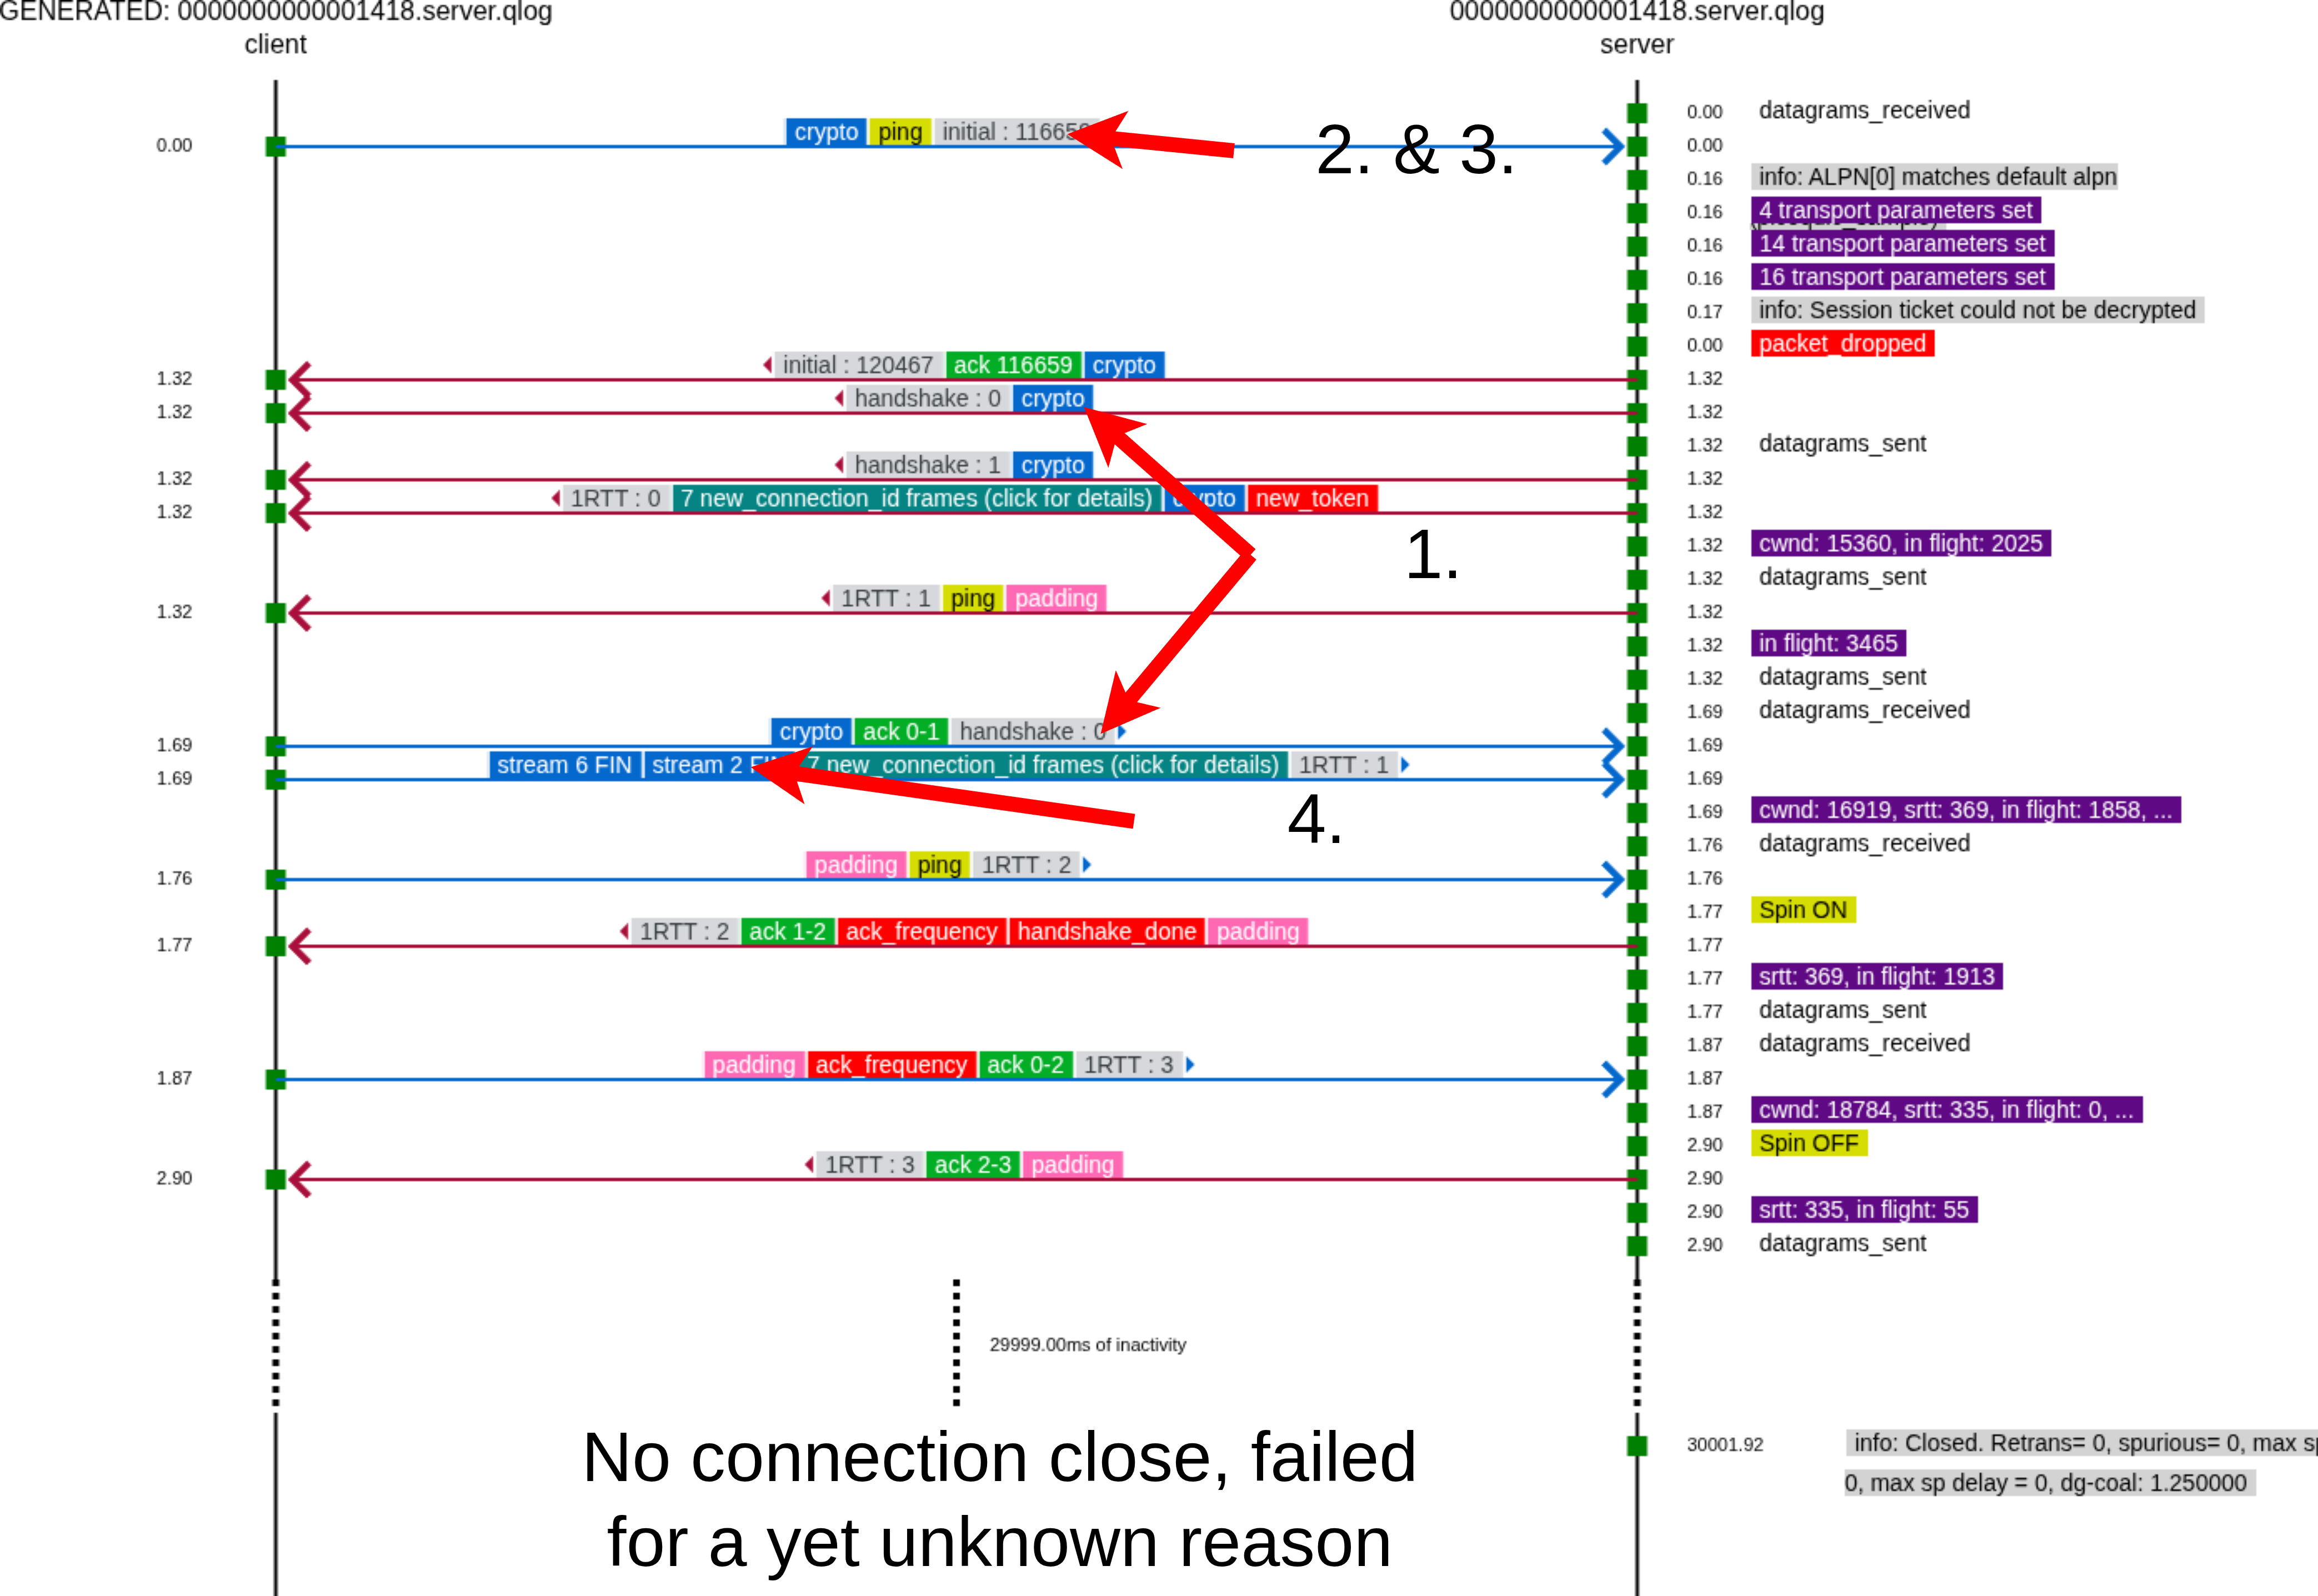
\includegraphics[width=\linewidth]{images/diagram.drawio.png}
    \caption{Marked Flow Diagram of Client <-> Server Connection}
    
\end{figure}


    


\end{document}